\documentclass{article}

\usepackage{Sweave}
\begin{document}
\Sconcordance{concordance:ensayo.tex:ensayo.Rnw:%
1 2 1 1 0 6 1 1 6 2 1 1 4 14 0 1 2 1 4 1 2 1 9 2 1}


En esta sección exploro cada índice. En esta sección exploro cada índice. En esta sección exploro cada índice. En esta sección exploro cada índice. En esta sección exploro cada índice. En esta sección exploro cada índice. En esta sección exploro cada índice. En esta sección exploro cada índice. En esta sección exploro cada índice.




No podemos hacer tabla de frecuencias, entonces sacamos solamente los estadisticos:

% Table created by stargazer v.5.2.2 by Marek Hlavac, Harvard University. E-mail: hlavac at fas.harvard.edu
% Date and time: vie., jun. 29, 2018 - 5:44:46 p.m.
\begin{table}[!htbp] \centering 
  \caption{Medidas estadísticas} 
  \label{stats} 
\begin{tabular}{@{\extracolsep{5pt}}lcc} 
\\[-1.8ex]\hline 
\hline \\[-1.8ex] 
Statistic & \multicolumn{1}{c}{N} & \multicolumn{1}{c}{Median} \\ 
\hline \\[-1.8ex] 
Población.Cabecera & 32 & 717,197 \\ 
Población.Resto & 32 & 268,111.5 \\ 
Población.Total & 32 & 1,028,429 \\ 
\hline \\[-1.8ex] 
\end{tabular} 
\end{table} \begin{figure}
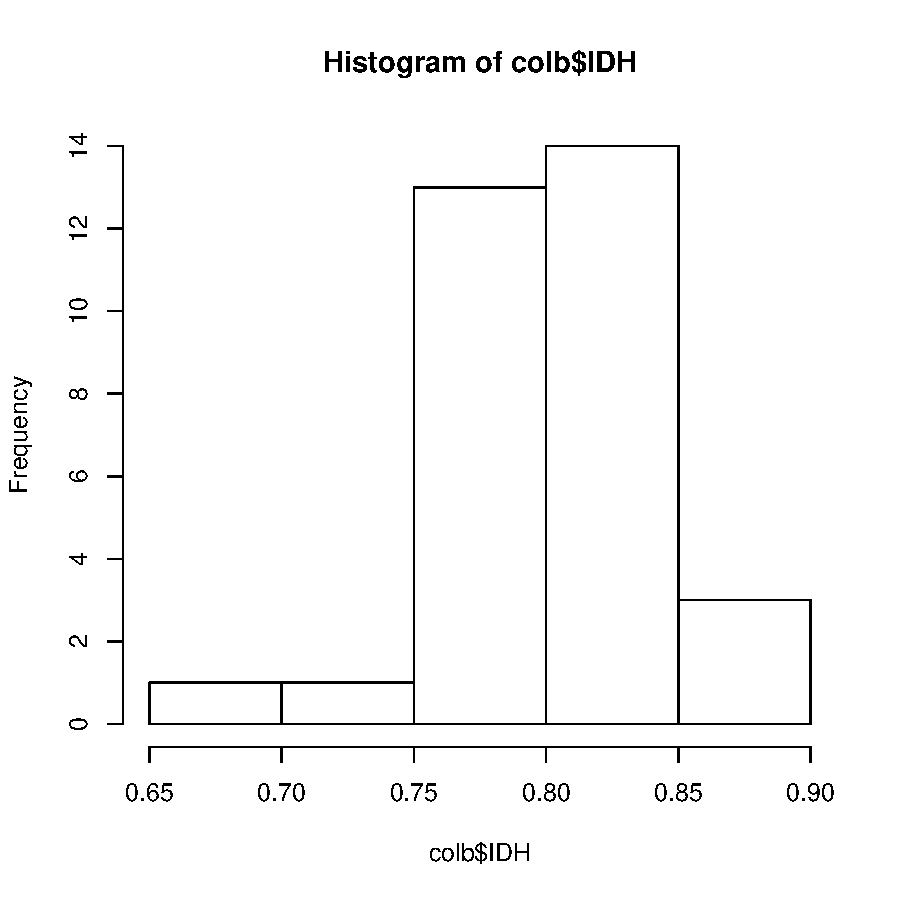
\includegraphics{ensayo-histogramas}
\end{figure}



\end{document}
